% Ergebnisse - Endergebnisse der Arbeit, Performance, Bilder (auf dpi achten, mind. 300), Kennkurven, Warps, weitere Leistungsmessungen bez. auf meine Arbeit
% -> ggf. Results and Discussion seperat halten
% Bedeutung der Ergebnisse (im Rahmen dessen was wissenschaftlich haltbar ist)
\chapter{Ergebnisse und Diskussion}\label{chap::resdisc}
Dieses Kapitel beinhaltet die Ergebnisse dieser Arbeit und eine anschließende Diskussion der Messwerte und der Umsetzung verschiedener Arbeitspakete.
Der erste Abschnitt behandelt dabei die Bildqualität und die gemessene Performanz der Implementierungen der Arbeitspakete aus Kapitel \ref{chap::design}.
Im zweiten Abschnitt werden diese diskutiert.

\section{Ergebnisse}\label{sec::results}
Der erste Abschnitt beinhaltet Ergebnissen der Implementierungen \emph{MDC} \ref{ss::MDC} und \emph{DDC} \ref{ss::DDC} sowie der ursprünglichen Implementierung des Raycasts \ref{ss::rc} aus Sicht der Bildqualität.
Der zweite Abschnitt beinhaltet gemessene Performanzleistungen der jeweiligen Implementierungen bei der Verwendung unterschiedlicher Transferfunktionen und Volumendaten.

\subsection{Bildqualität}
Im folgenden werden zu den Implementierungen \emph{MDC}, \emph{DDC} und als Vergleich zur Ursprünglichen Implementierung Screenshots gezeigt, welche die Bildqualität der Implementierungen darstellen sollen.
Dies wird anhand von drei verschiedenen Volumen mit jeweils einer Transferfunktion dargestellt.
Für jedes der Volumen wird jeweils das Bild in normaler Auflösung, welche mit der ursprünglichen Implementierung berechnet wurde sowie das Ergebnis der Berechnung des Bildes durch \emph{MDC} und \emph{DDC} gezeigt.
Bei den Berechnungen durch \emph{MDC} und \emph{DDC} werden die jeweils verwendeten Parameter der Berechnung angegeben.

% \subsubsection{Bonsai}
\begin{landscape}
	\begin{figure}
		\centering
		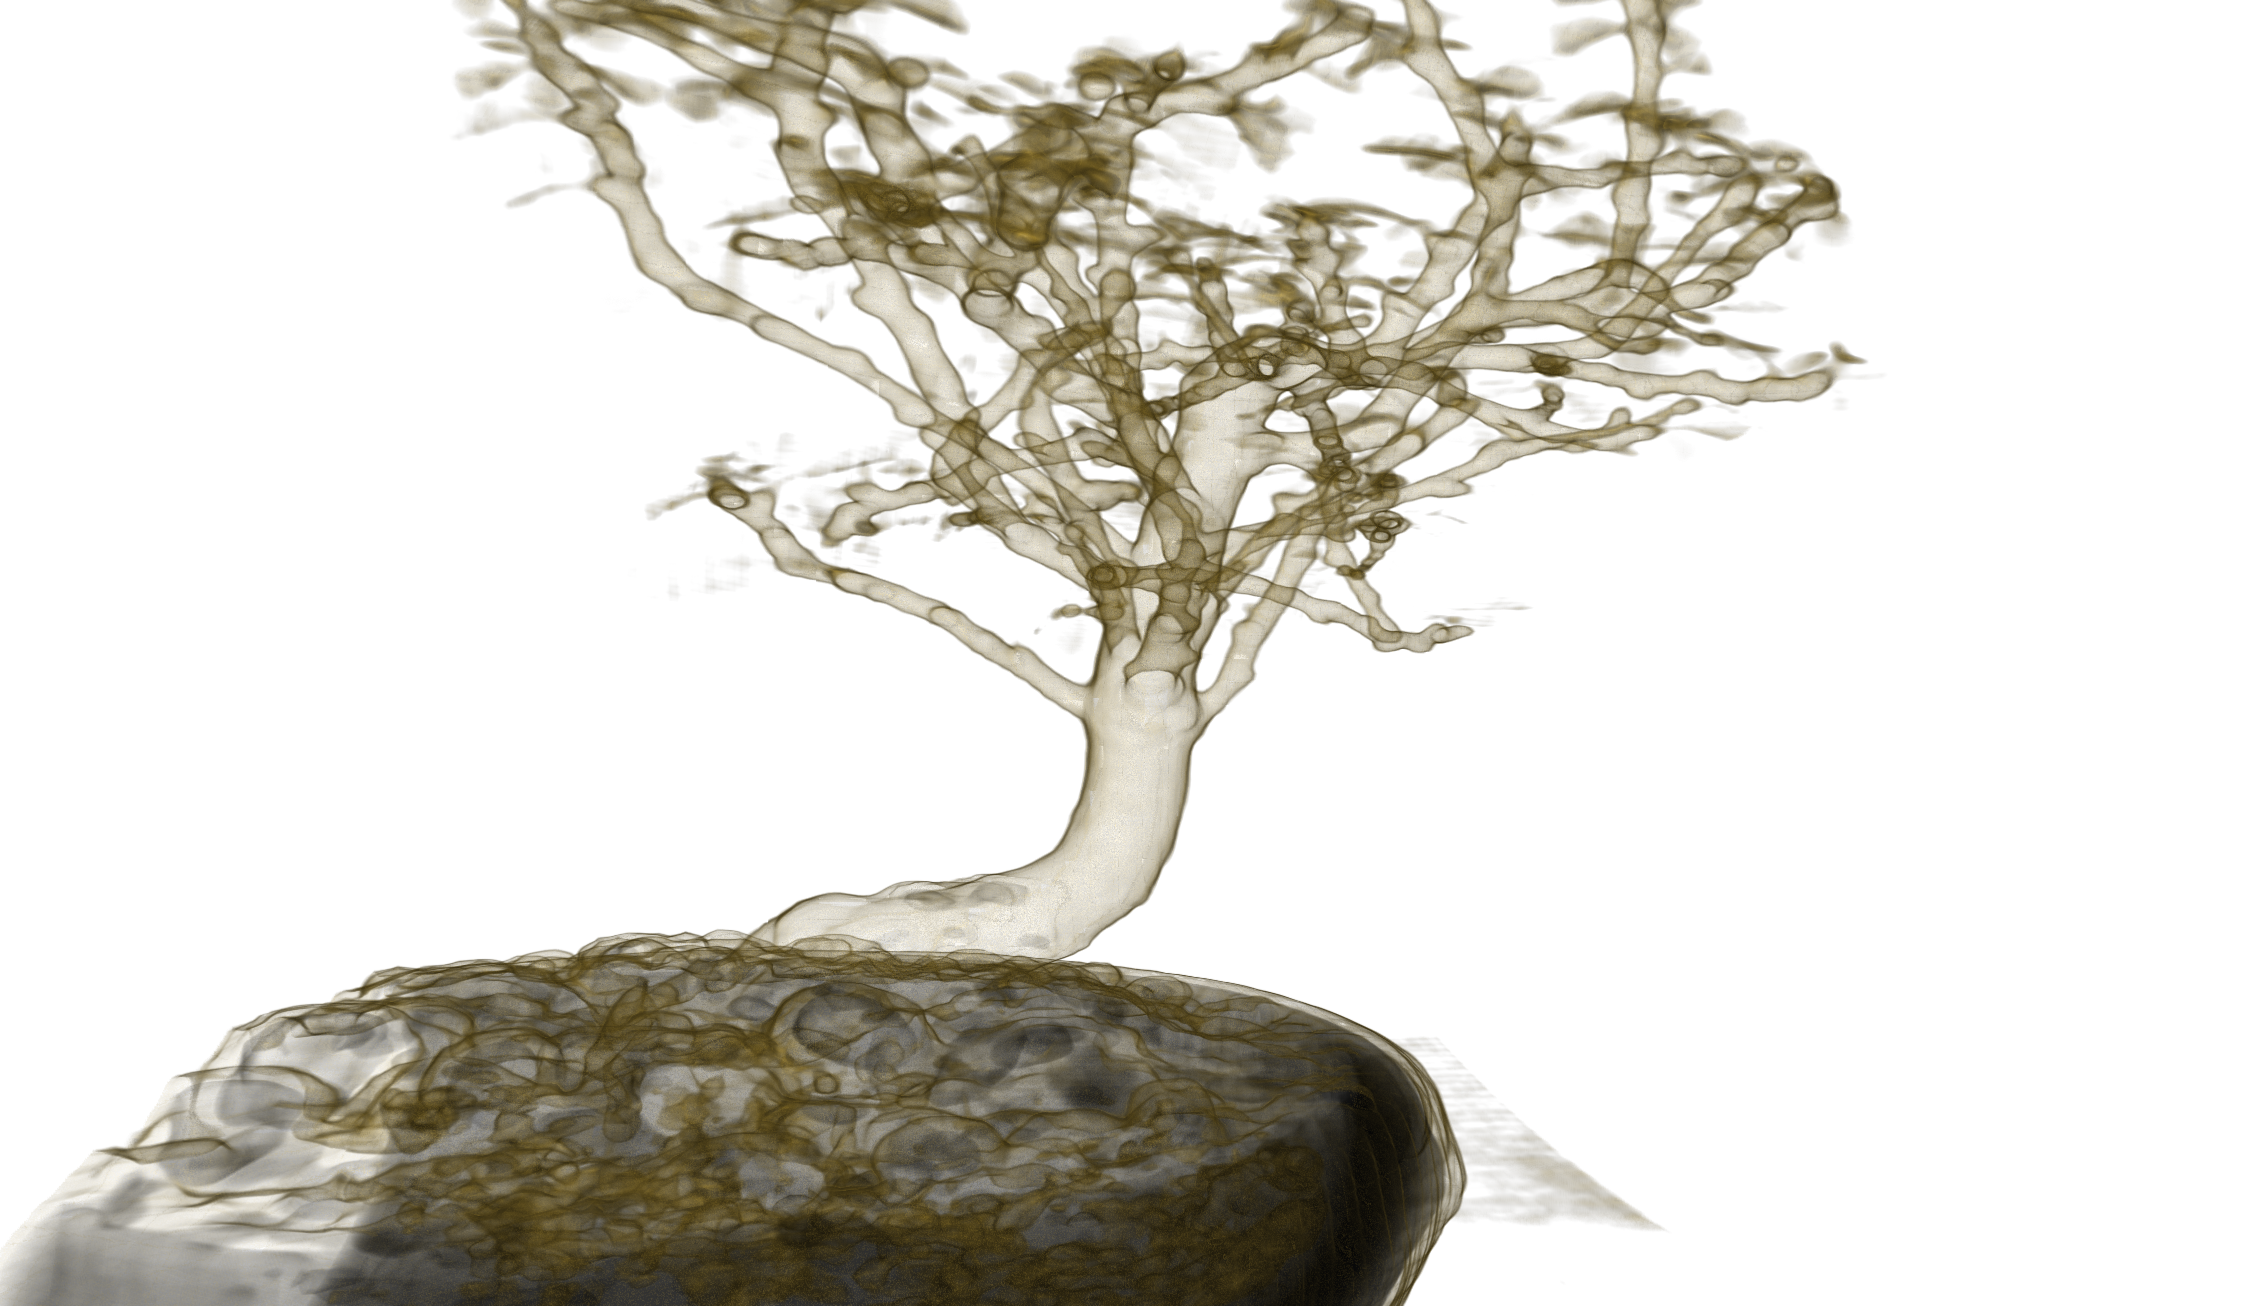
\includegraphics[width=\textheight]{../../Grafiken/results/picture_quality/bonsai/Standard_img-1_Ray-1-5.png}
		\caption{Volumen Bonsai mit ursprünglichem Raycast berechnet.}
		\label{fig::res::bon_st}
	\end{figure}
\end{landscape}

\begin{landscape}
	\begin{figure}
		\centering
		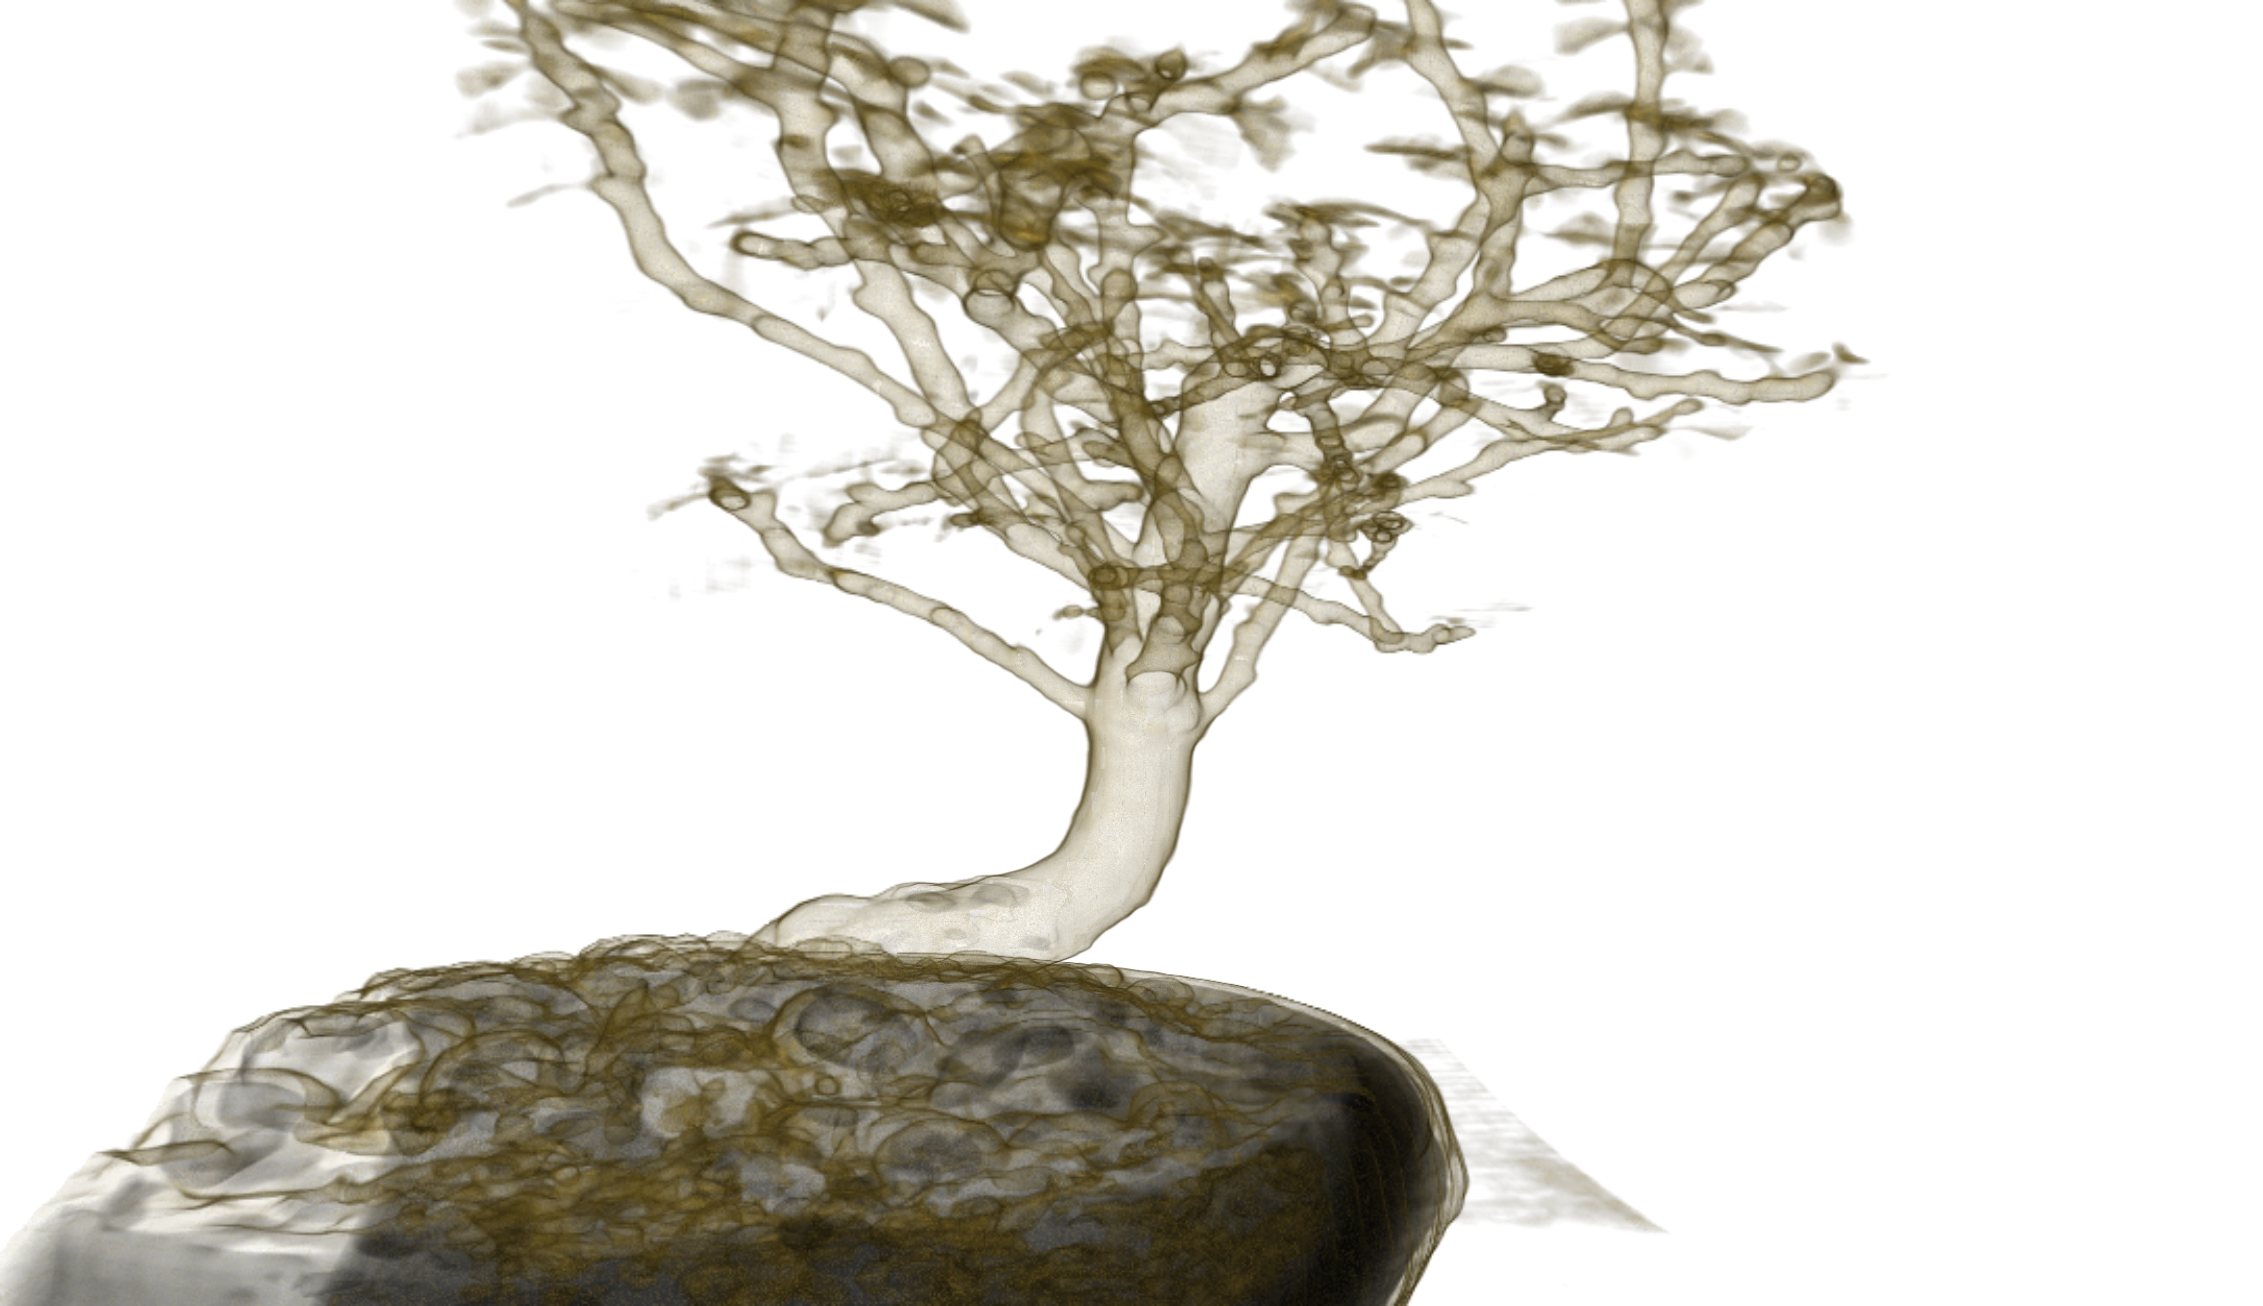
\includegraphics[width=1\textheight]{../../Grafiken/results/picture_quality/bonsai/MDC_img-0-96_ray-1-5.png}
		\caption{Volumen Bonsai mit \emph{MDC} Raycast berechnet.}
		\label{fig::res::bon_mdc}
	\end{figure}
\end{landscape}

\begin{landscape}
	\begin{figure}
		\centering
		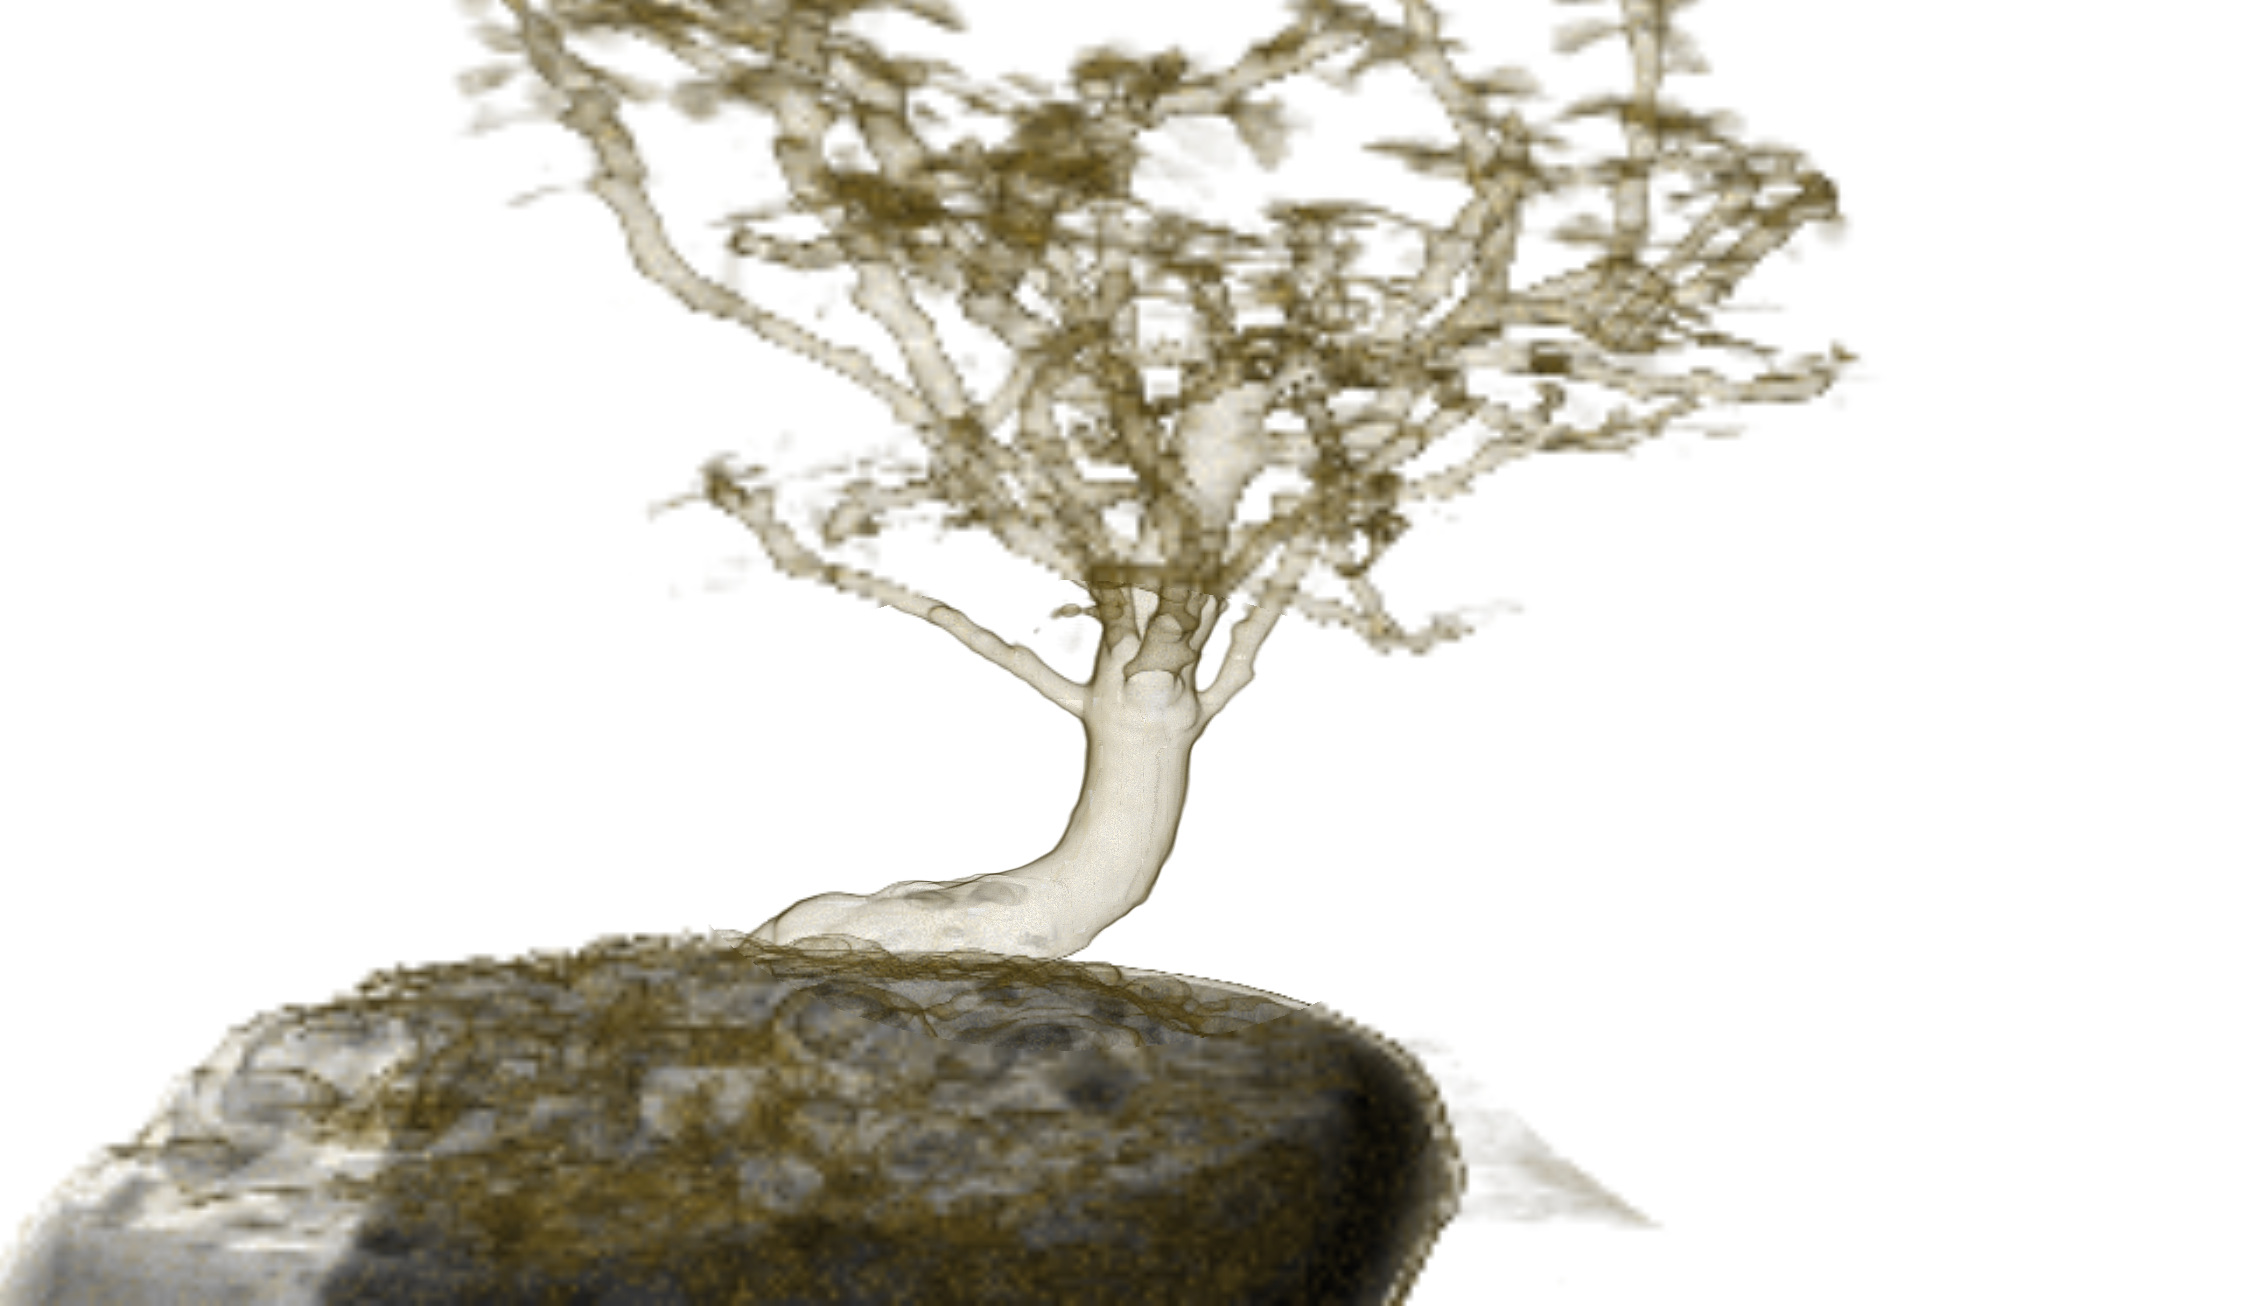
\includegraphics[width=1\textheight]{../../Grafiken/results/picture_quality/bonsai/DDC_img-1_ray-1-5.png}
		\caption{Volumen Bonsai mit \emph{DDC} Raycast berechnet.}
		\label{fig::res::bon_ddc}
	\end{figure}
\end{landscape}


% \subsubsection{Chameleon}
\begin{landscape}
	\begin{figure}
		\centering
		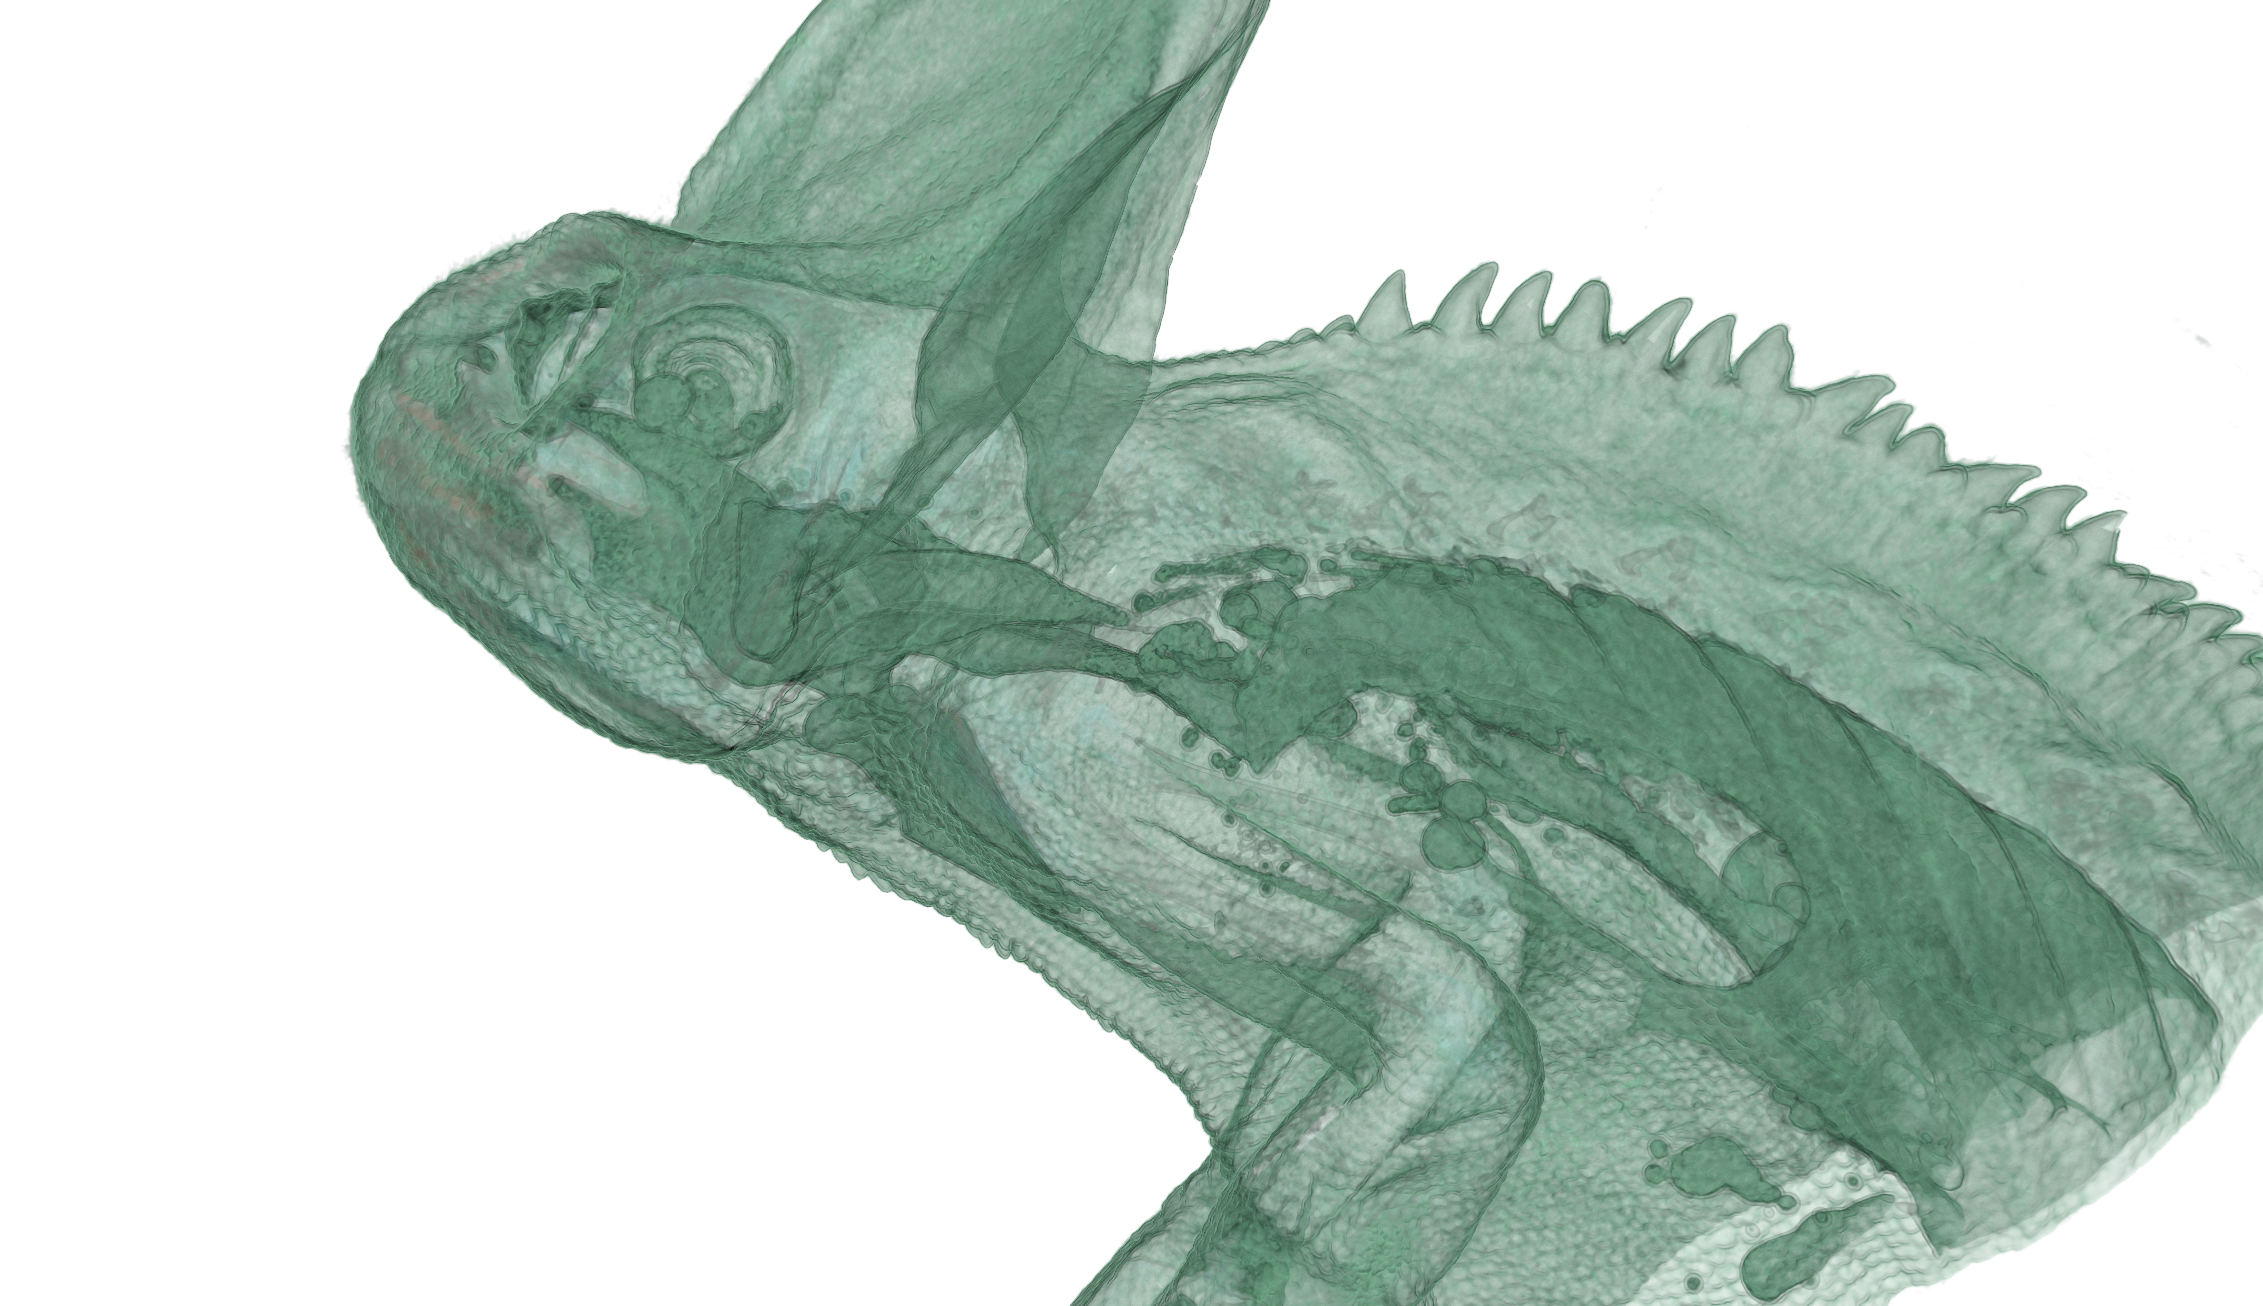
\includegraphics[width=1\textheight]{../../Grafiken/results/picture_quality/chameleon/Standard_img-1_Ray-1-5.png}
		\caption{Volumen Chameleon mit ursprünglichem Raycast berechnet.}
		\label{fig::res::cam_st}
	\end{figure}
\end{landscape}

\begin{landscape}
	\begin{figure}
		\centering
		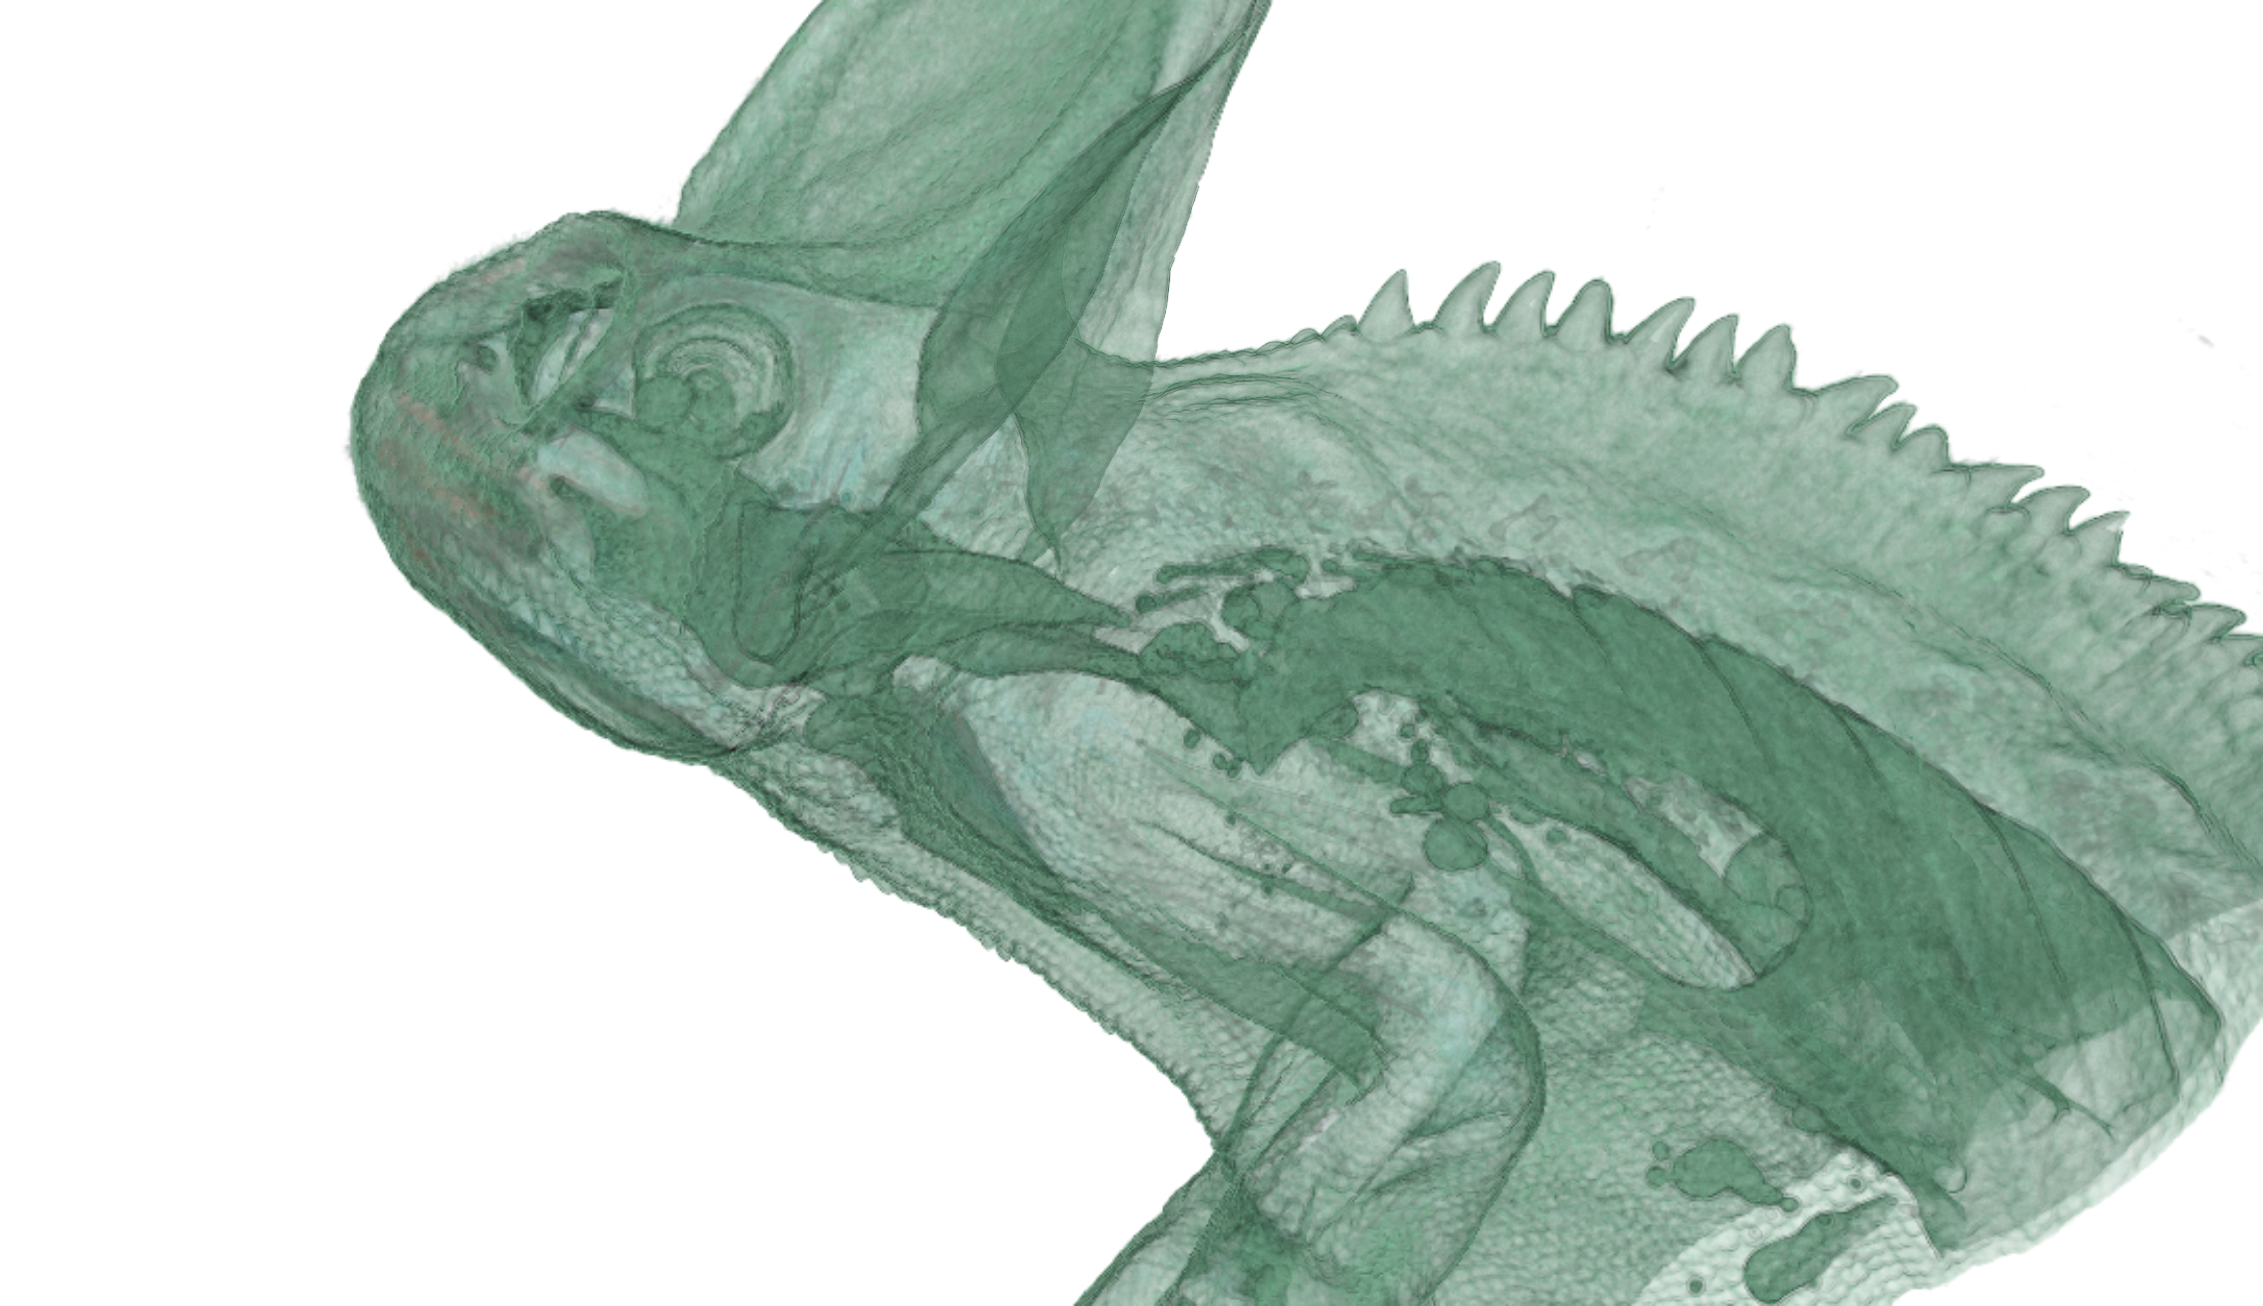
\includegraphics[width=1\textheight]{../../Grafiken/results/picture_quality/chameleon/MDC_img-0-96_ray-1-5.png}
		\caption{Volumen Chameleon mit \emph{MDC} Raycast berechnet.}
		\label{fig::res::cam_mdc}
	\end{figure}
\end{landscape}

\begin{landscape}
	\begin{figure}
		\centering
		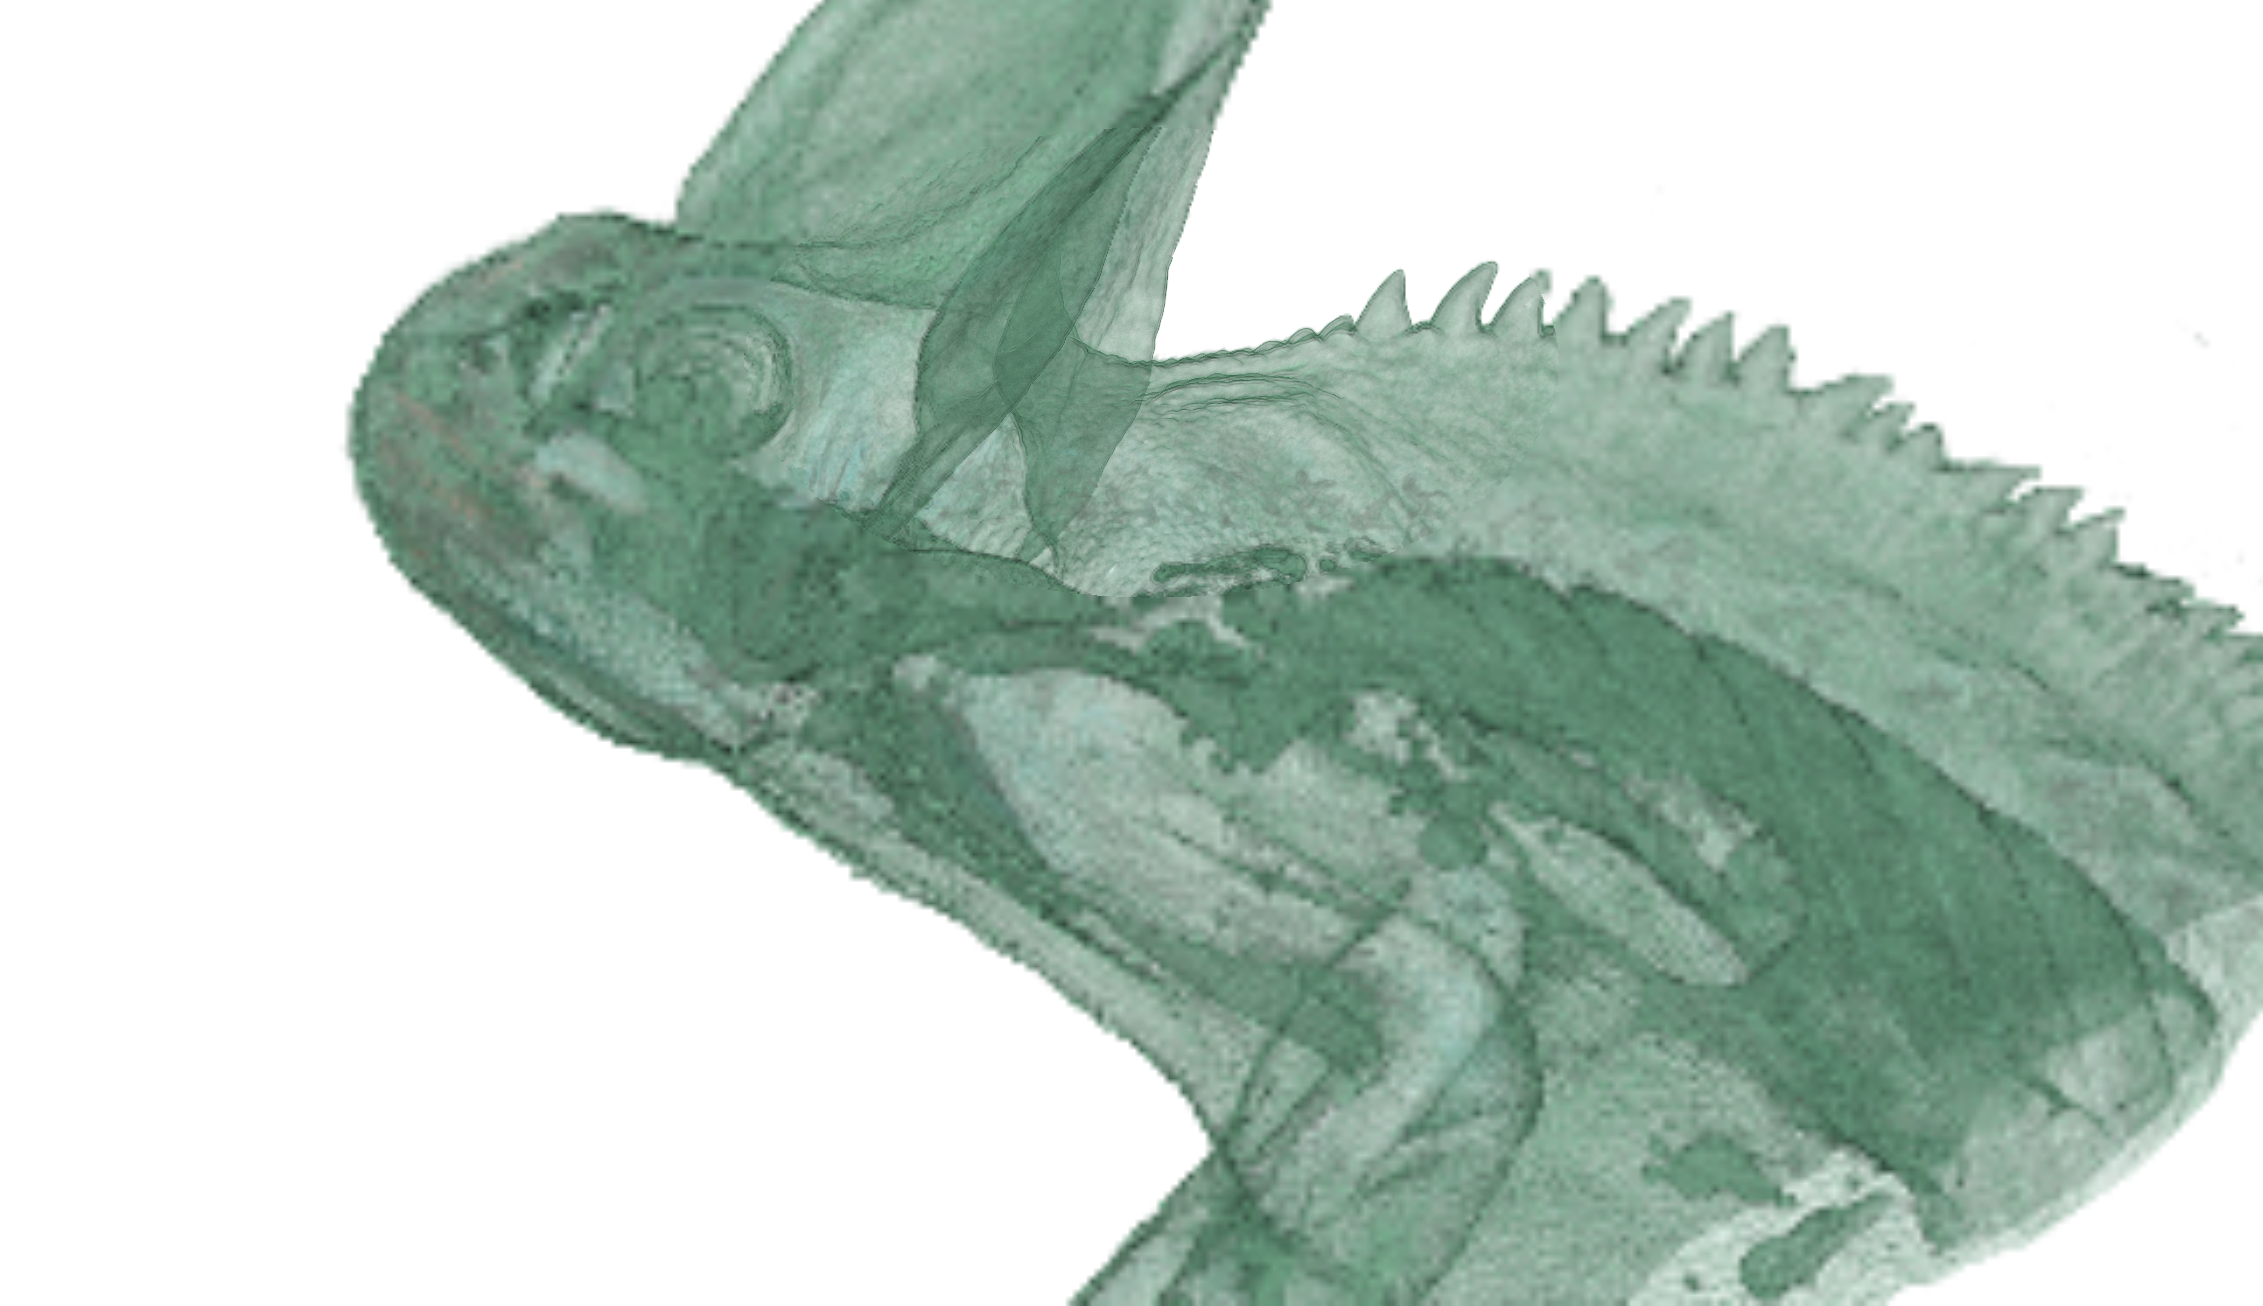
\includegraphics[width=1\textheight]{../../Grafiken/results/picture_quality/chameleon/DDC_img-1_ray-1-5.png}
		\caption{Volumen Chameleon mit \emph{DDC} Raycast berechnet.}
		\label{fig::res::cam_ddc}
	\end{figure}
\end{landscape}


% \subsubsection{Hoatzin}
\begin{landscape}
	\begin{figure}
		\centering
		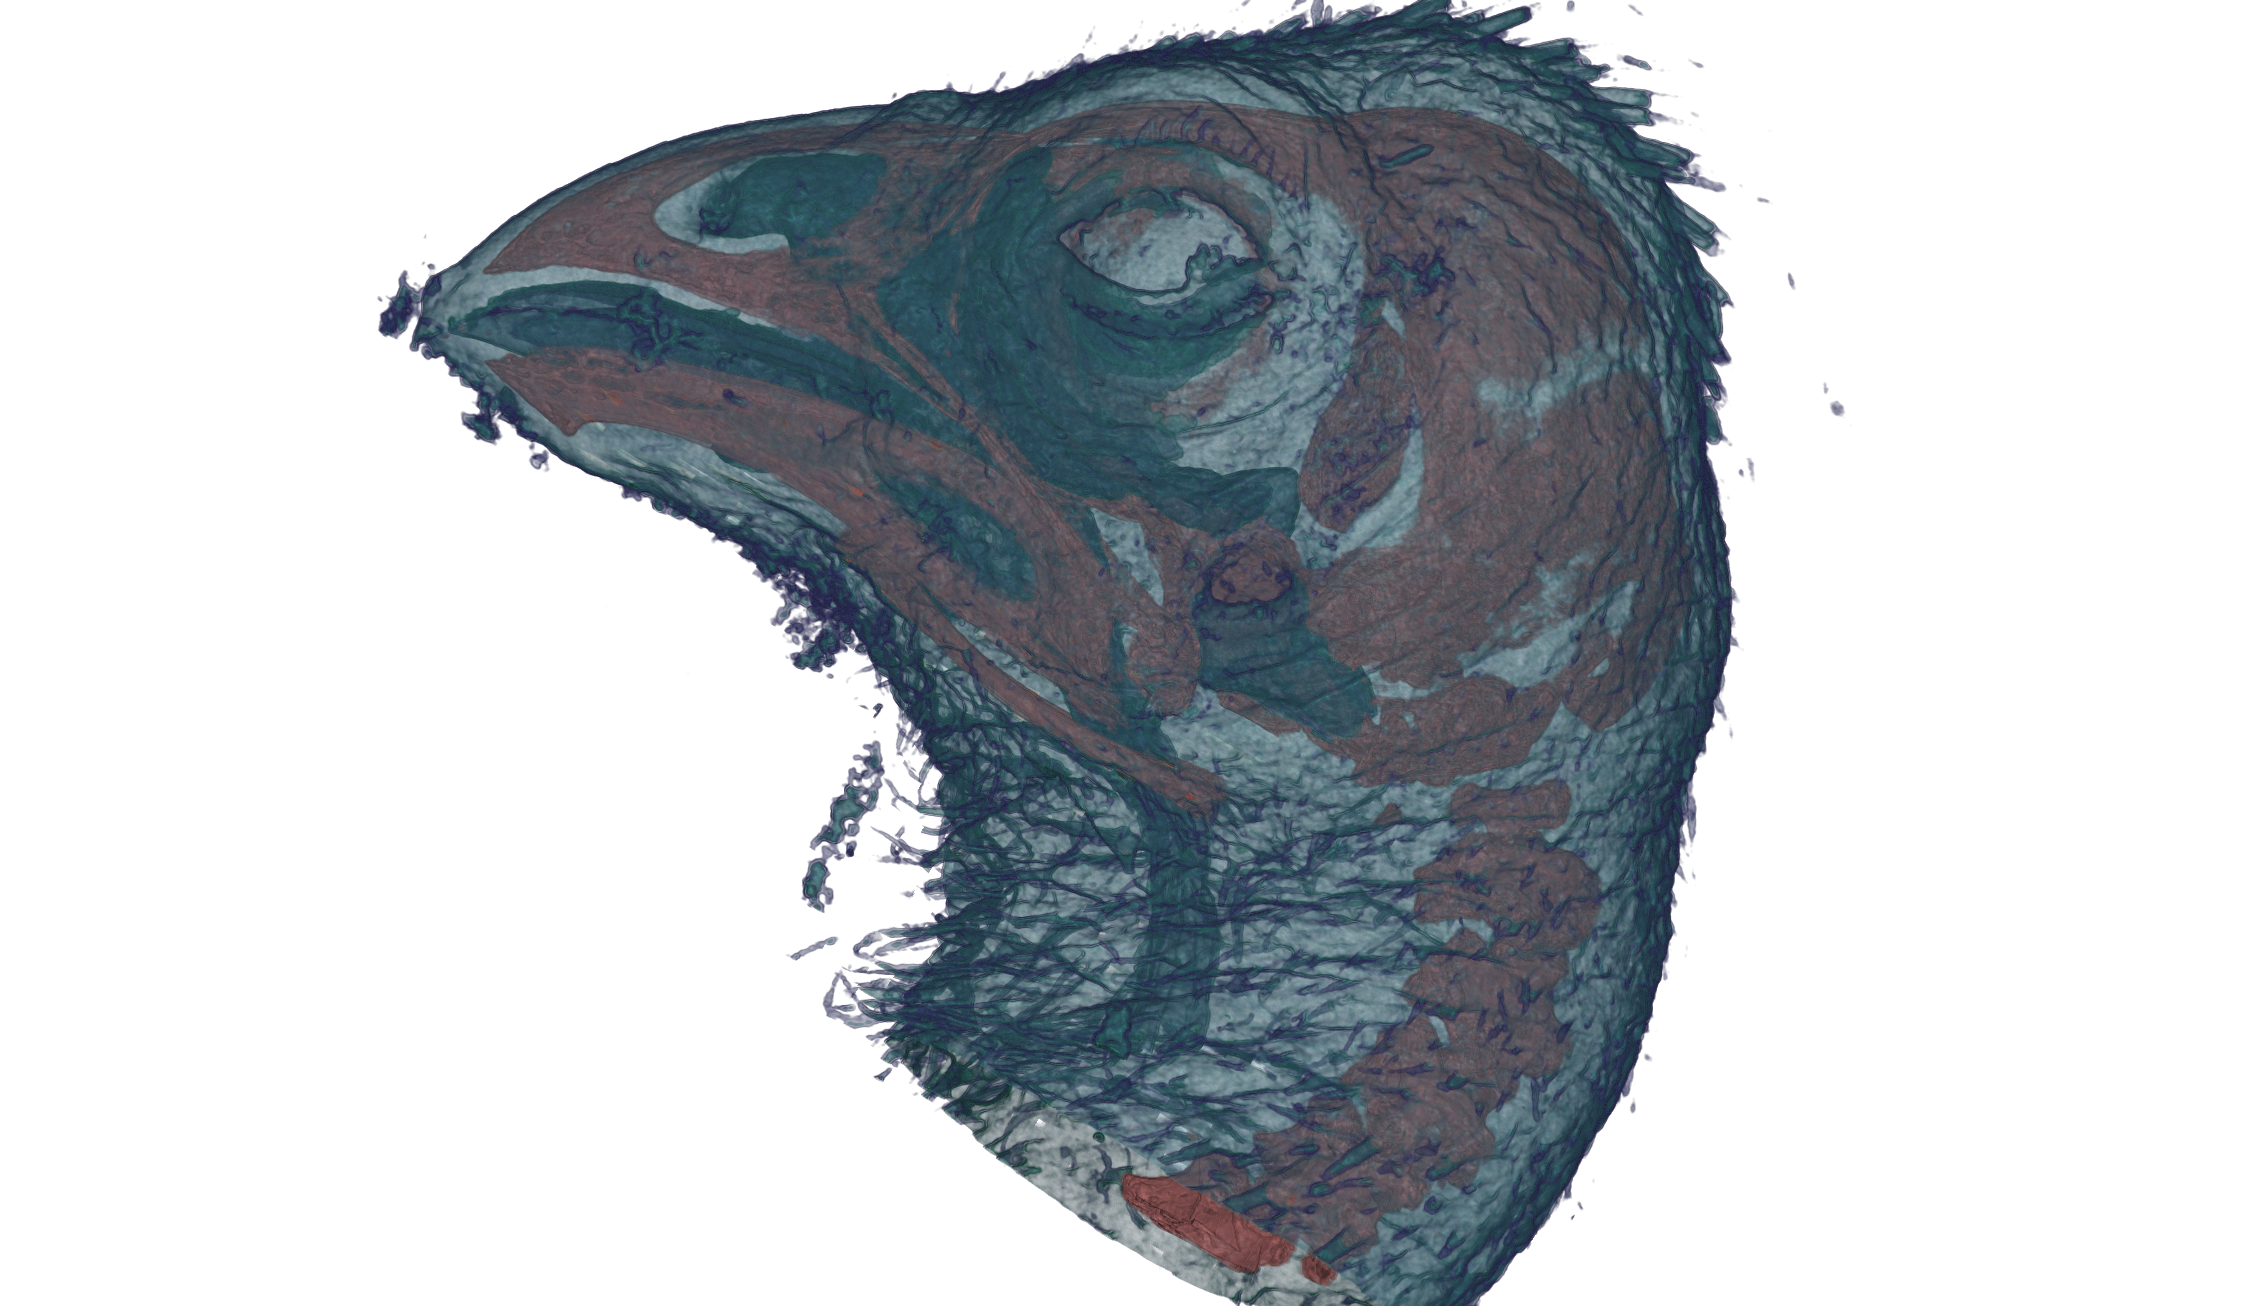
\includegraphics[width=1\textheight]{../../Grafiken/results/picture_quality/hoatzin/Standard_img-1_Ray-1-5.png}
		\caption{Volumen Hoatzin mit ursprünglichem Raycast berechnet.}
		\label{fig::res::hoa_st}
	\end{figure}
\end{landscape}

\begin{landscape}
	\begin{figure}
		\centering
		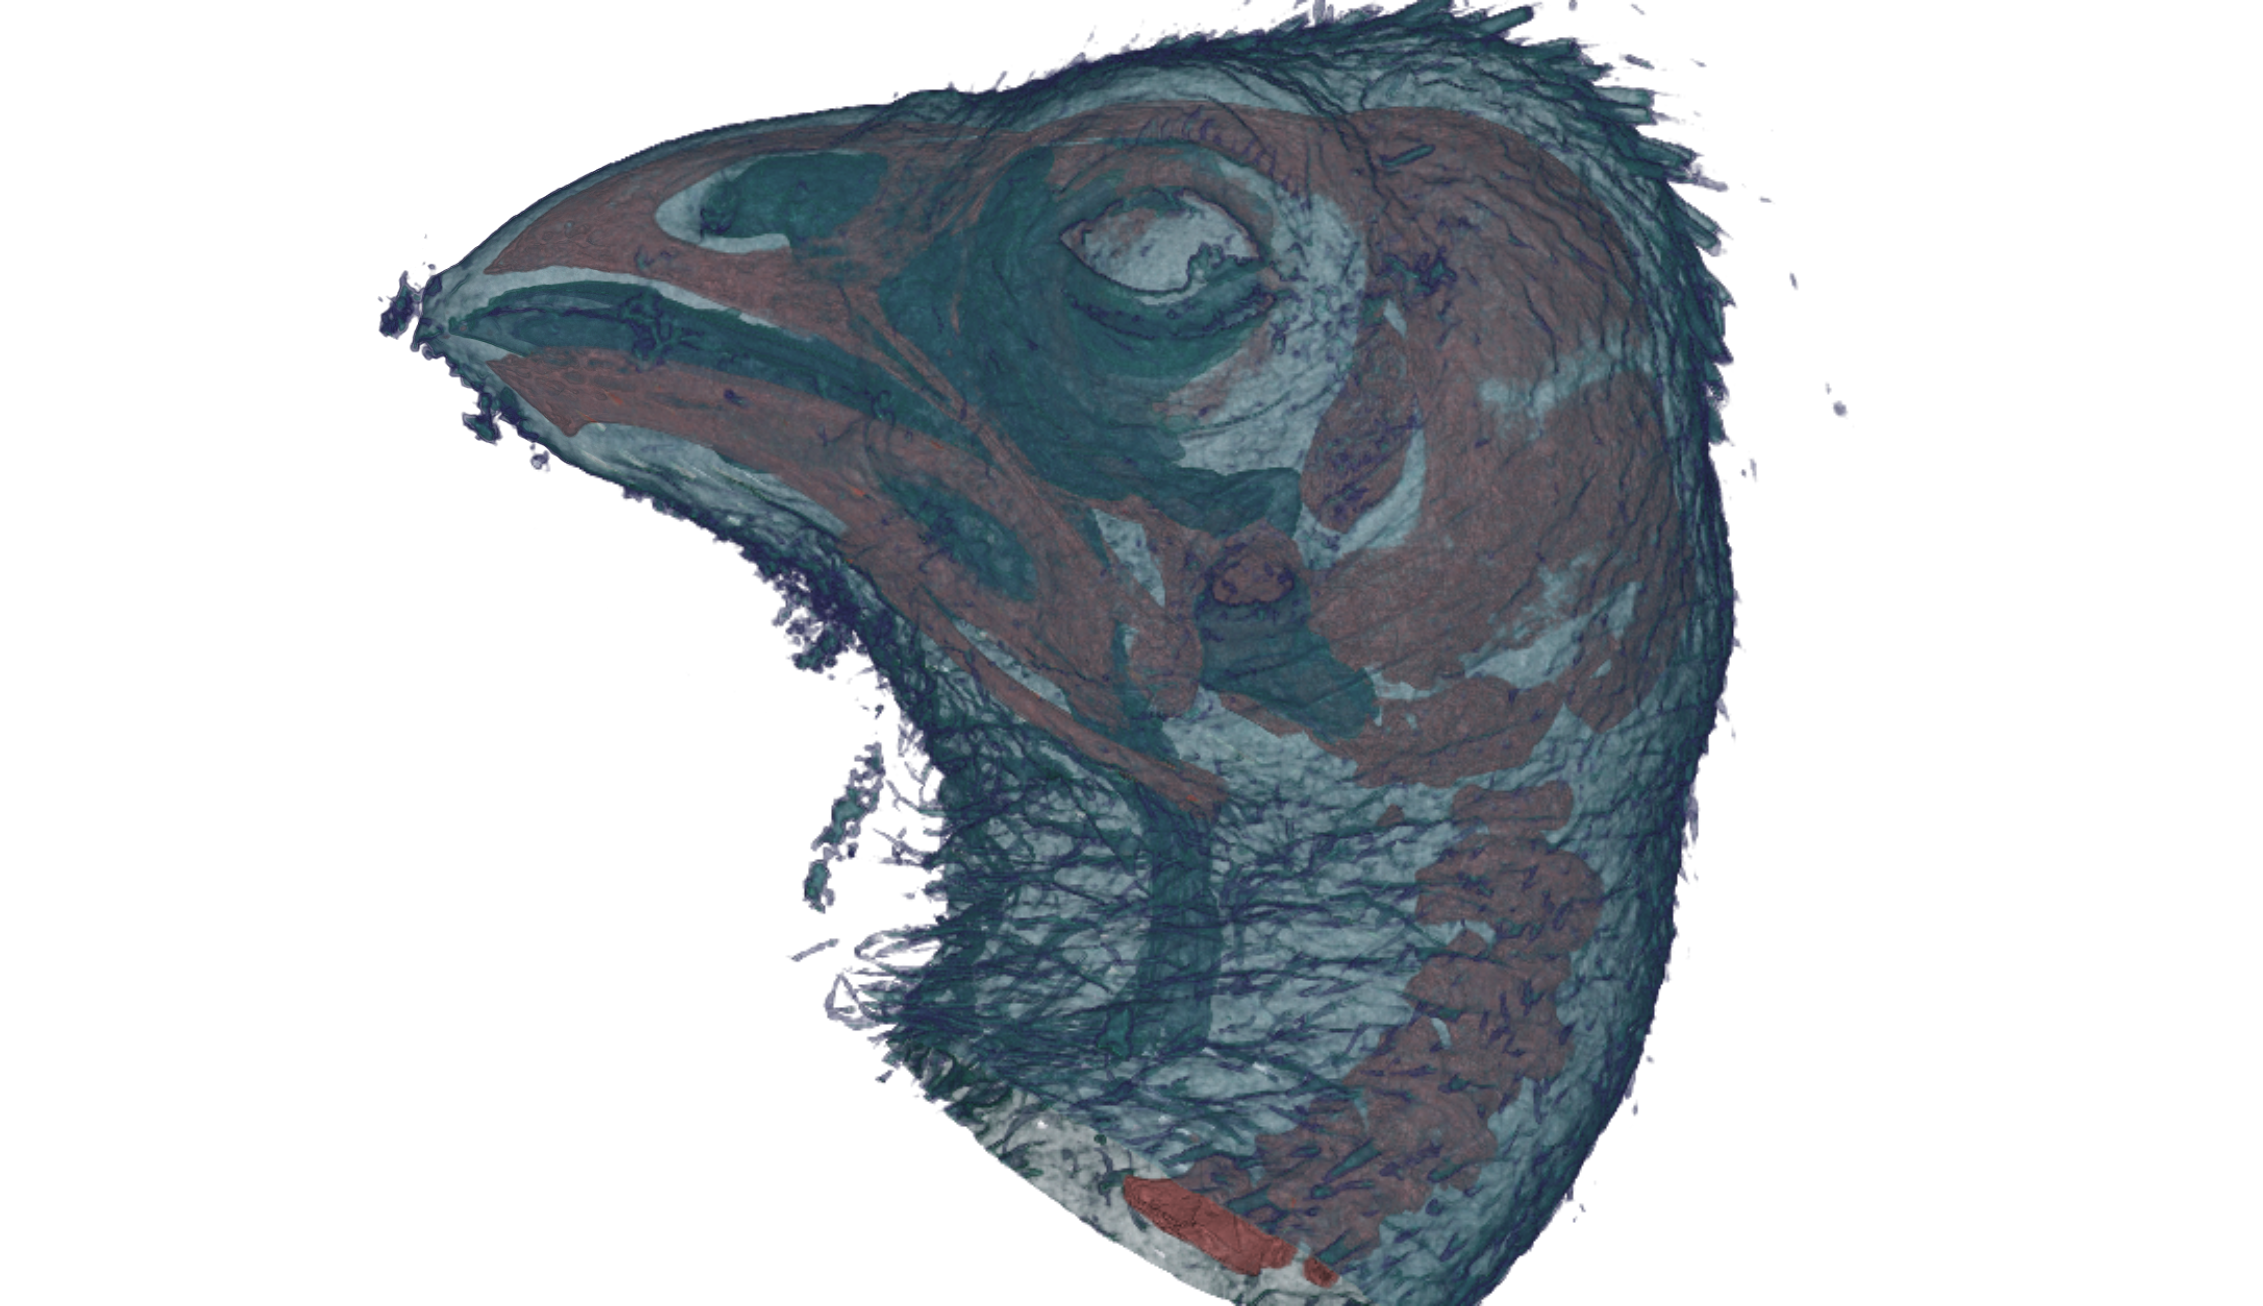
\includegraphics[width=1\textheight]{../../Grafiken/results/picture_quality/hoatzin/MDC_img-0-96_ray-1-5.png}
		\caption{Volumen Hoatzin mit \emph{MDC} Raycast berechnet.}
		\label{fig::res::hoa_mdc}
	\end{figure}
\end{landscape}

\begin{landscape}
	\begin{figure}
		\centering
		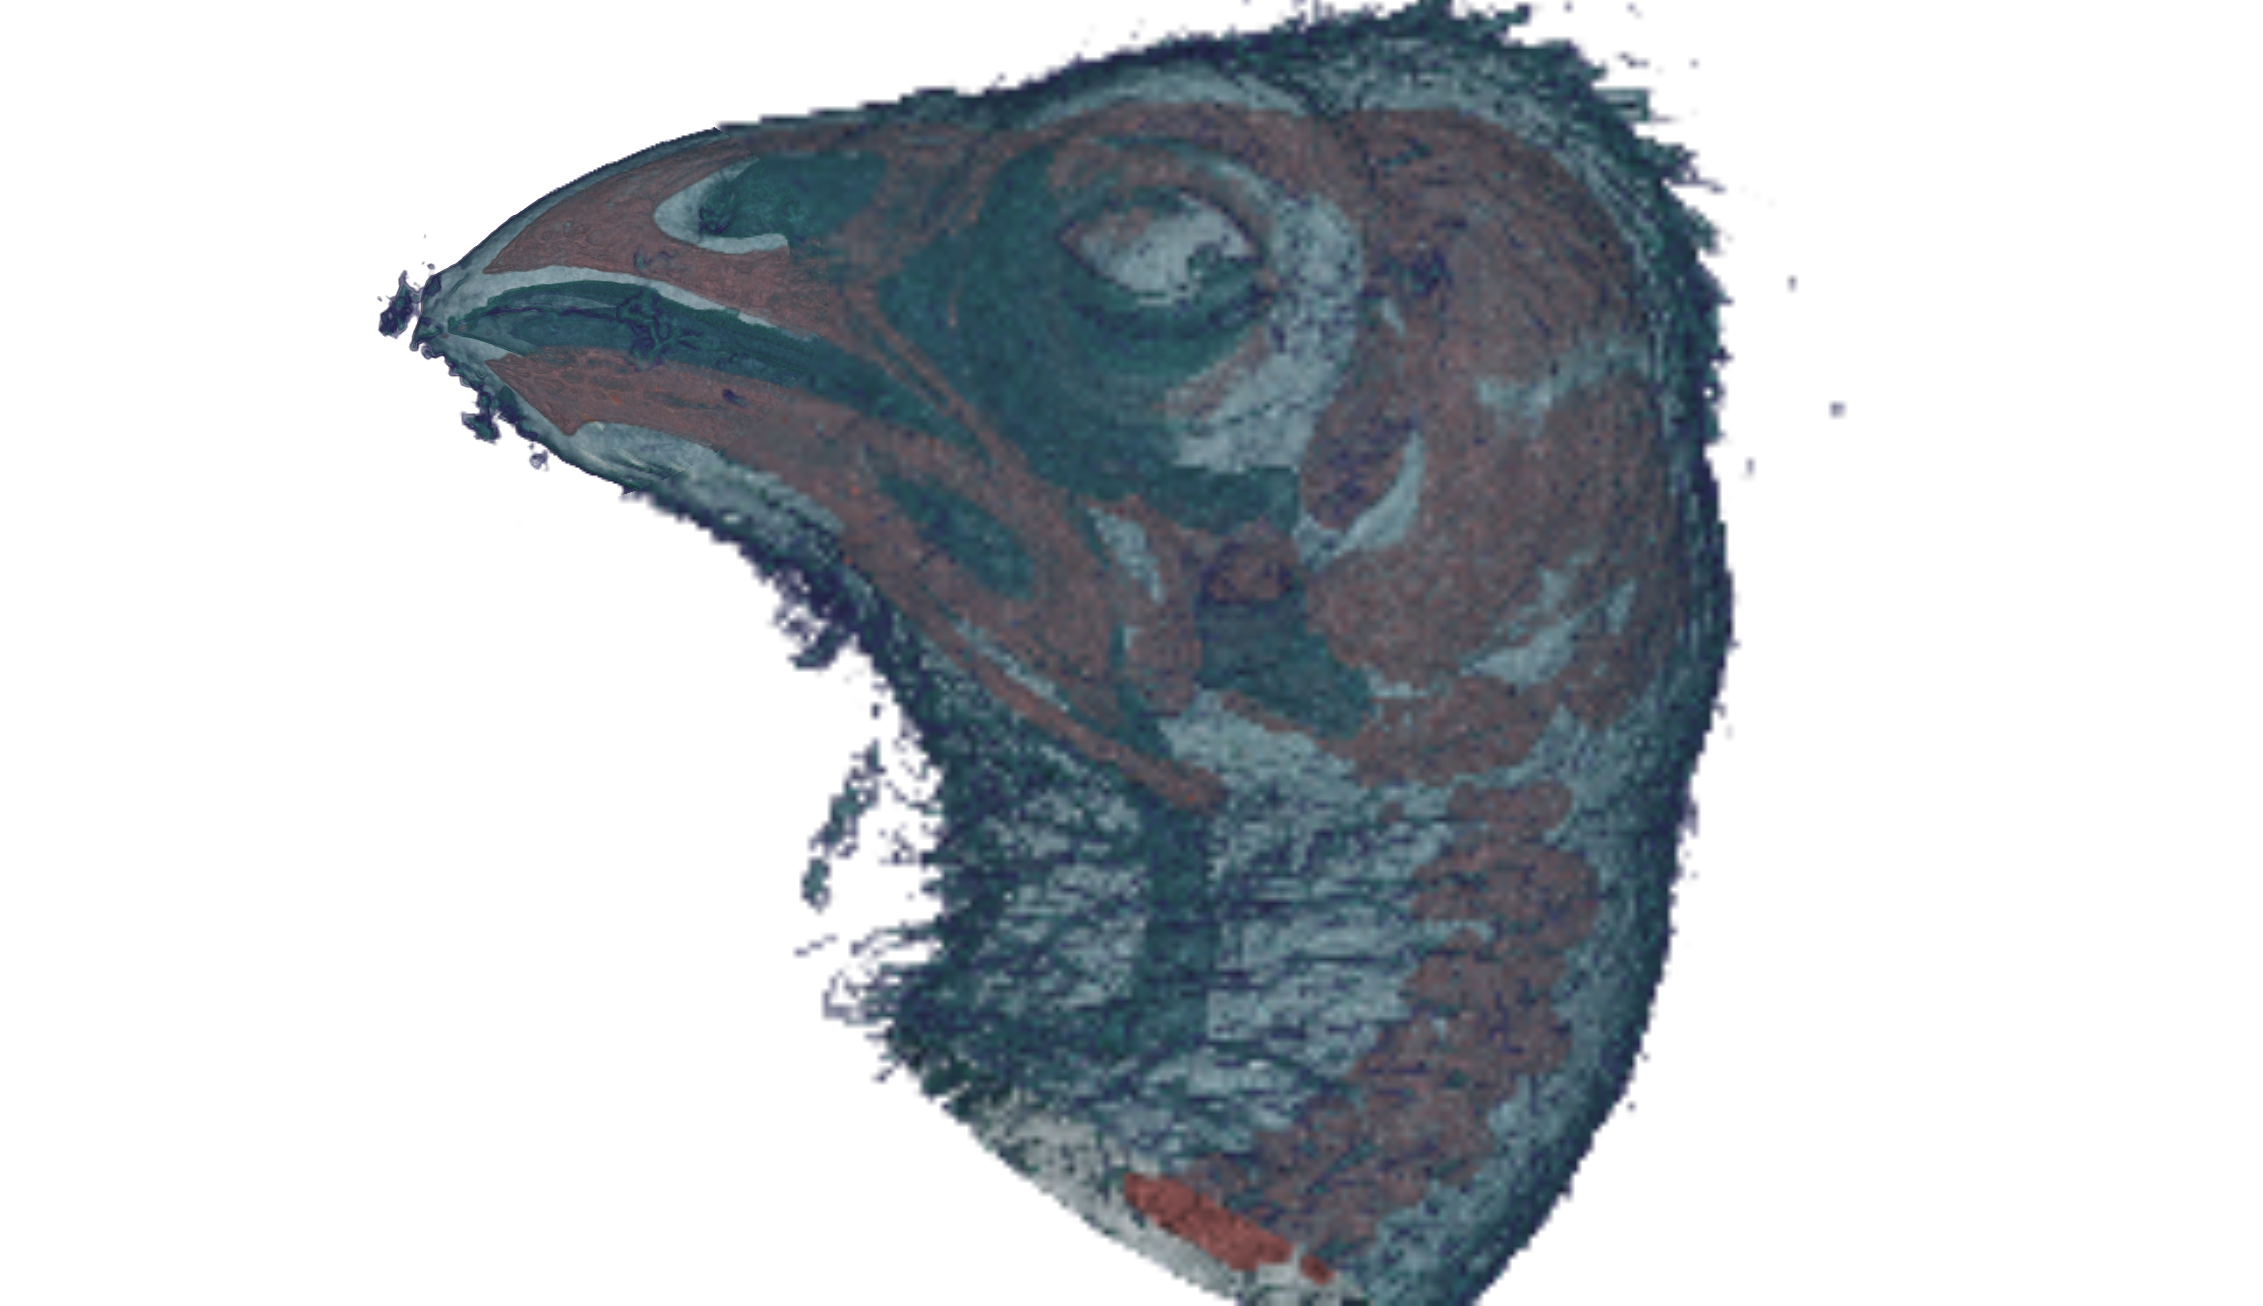
\includegraphics[width=1\textheight]{../../Grafiken/results/picture_quality/hoatzin/DDC_img-1_ray-1-5.png}
		\caption{Volumen Hoatzin mit \emph{DDC} Raycast berechnet.}
		\label{fig::res::hoa_ddc}
	\end{figure}
\end{landscape}


\subsection{Performanz}





\todo{Messbare Ergebnisse der Arbeit. (Performanzmessungen..).}

\section*{Diskussion}\label{sec::disc}
\todo{Diskussion und Bedeutung der Ergebnisse.}